%%%%%%%%%%%%%%%%%%%%%%%%%%%%%%%%%%%%%%%%%%%%%%%%%%%%%%%%%%%%%%%%%%%%%%%%%%%%%%%%
% IEEE Conference Template for CSE356 IoT Project
% - Structured for the 10-step IoT Design Methodology
% - Configured for BibTeX (references.bib) and a figures folder
%%%%%%%%%%%%%%%%%%%%%%%%%%%%%%%%%%%%%%%%%%%%%%%%%%%%%%%%%%%%%%%%%%%%%%%%%%%%%%%%

\documentclass[conference]{IEEEtran}
\IEEEoverridecommandlockouts
% The preceding line is only needed to identify funding in the first footnote. If that is unneeded, please comment it out.
\usepackage{cite}
\usepackage{booktabs}
\usepackage{amsmath,amssymb,amsfonts}
\usepackage{algorithmic}
\usepackage{graphicx}
\usepackage{textcomp}
\usepackage{xcolor}
\usepackage{tabularx}
\def\BibTeX{{\rm B\kern-.05em{\sc i\kern-.025em b}\kern-.08em
    T\kern-.1667em\lower.7ex\hbox{E}\kern-.125emX}}

% Set the path for your figures directory
\graphicspath{{figures/}}

\usepackage{tikz}
\usetikzlibrary{arrows.meta,positioning,shadows.blur}

\definecolor{primary}{HTML}{0A84FF}
\definecolor{accent}{HTML}{FF453A}
\definecolor{ink}{HTML}{0A0A0A}

\begin{document}

% --- TITLE ---
\title{Design and Prototyping of an IoT Smart Home Security System\\
}

% --- TEAM'S NAMES ---
\author{\IEEEauthorblockN{Hamsa Ahmad}
\IEEEauthorblockA{\textit{Computer and Systems Eng. Dept.} \\
\textit{Ain Shams University}\\
Cairo, Egypt \\
20P1874@eng.asu.edu.eg}
\and
\IEEEauthorblockN{Student Name 2}
\IEEEauthorblockA{\textit{Computer and Systems Eng. Dept.} \\
\textit{Ain Shams University}\\
Cairo, Egypt \\
2@eng.asu.edu.eg}
\and
\IEEEauthorblockN{Student Name 3}
\IEEEauthorblockA{\textit{Computer and Systems Eng. Dept.} \\
\textit{Ain Shams University}\\
Cairo, Egypt \\
2@eng.asu.edu.eg}
\and
\IEEEauthorblockN{Student Name 4}
\IEEEauthorblockA{\textit{Computer and Systems Eng. Dept.} \\
\textit{Ain Shams University}\\
Cairo, Egypt \\
2@eng.asu.edu.eg}
\and
\IEEEauthorblockN{Belal Anas Awad}
\IEEEauthorblockA{\textit{Computer and Systems Eng. Dept.} \\
\textit{Ain Shams University}\\
Cairo, Egypt \\
21P0072@eng.asu.edu.eg}
}

\maketitle

% --- ABSTRACT AND KEYWORDS ---
\begin{abstract}
This paper presents the complete 10-step design methodology for an IoT-based Smart Home Security System. The system is designed to detect unauthorized access through a network of sensors, capture evidence using cameras, and provide real-time alerts to the homeowner. The design covers all aspects from requirement analysis and system modeling to the specification of devices, services, and applications, culminating in a comprehensive blueprint for implementation and simulation.
\end{abstract}

\begin{IEEEkeywords}
Internet of Things, IoT, Smart Home, Security System, System Design, Cisco Packet Tracer
\end{IEEEkeywords}


%%%%%%%%%%%%%%%%%%%%%%%%%%%%%%%%%%%%%%%%%%%%%%%%%%%%%%%%%%%%%%%%%%%%%%%%%%%%%%%%
% --- START OF THE PROJECT REPORT BODY ---
%%%%%%%%%%%%%%%%%%%%%%%%%%%%%%%%%%%%%%%%%%%%%%%%%%%%%%%%%%%%%%%%%%%%%%%%%%%%%%%%

\section{Introduction}

The Internet of Things (IoT) has emerged as a transformative technology, connecting everyday objects to the internet and enabling intelligent automation and monitoring. One of the most impactful applications of IoT is in the domain of smart home systems, where connected devices enhance convenience, energy efficiency, and security. Home security, in particular, has seen significant innovation through IoT, moving from traditional isolated alarm systems to interconnected, responsive networks that provide homeowners with real-time awareness and control.

This paper details the design of an IoT-based Smart Home Security System. The primary objective is to create a robust and reliable system that detects potential intrusions and promptly alerts the homeowner. To ensure a thorough and systematic design, we adhere to the 10-step IoT design methodology, covering all aspects from initial requirements to application development. The following sections will elaborate on each step of this methodology, providing a complete blueprint for the system's architecture and functionality.


\section{IoT System Design Methodology}
This section details the design of the Smart Home Security System following the prescribed 10-step methodology.

% --- STEP 1 ---
\subsection{Step 1: Purpose \& Requirements Specification}
The primary purpose of this IoT system is to enhance home security by providing real-time detection of unauthorized entry or suspicious activity and notifying homeowners immediately. This system aims to be a proactive deterrent and a reliable monitoring tool, offering peace of mind to the user by integrating physical sensors with a smart notification platform.
\subsubsection{\textbf{Functional Requirements:}}
\begin{itemize}
    \item \textbf{Door/Window Monitoring:} The system must use magnetic sensors to detect when a door or window is opened and register this as a potential intrusion event.
    \item \textbf{Motion Detection:} PIR motion sensors must be able to detect human movement within designated areas of the home.
    \item \textbf{Camera Integration:} The system must be able to trigger a camera to capture images or video footage upon detecting a security event (e.g., a door opening or motion).
    \item \textbf{Real-time Alerts:} The system must send immediate notifications (e.g., push notifications or SMS) to the homeowner's mobile application when an event is detected.
    \item \textbf{Remote Control:} The homeowner must have the ability to arm or disarm the system and remotely control connected devices, such as activating a siren or turning on lights.
    \item \textbf{Monitoring Dashboard:} The mobile application must provide a live view of all sensor statuses and a log of past events.
\end{itemize}
\subsubsection{Non-Functional Requirements:}
\begin{itemize}
    \item \textbf{High Reliability:} The system must be highly reliable with a low rate of false alarms to maintain user trust.
    \item \textbf{Secure Communication:} All data transmission between sensors, the IoT hub, and the cloud must be encrypted to prevent eavesdropping or tampering.
    \item \textbf{Scalability}: The system must be designed to easily accommodate additional sensors, cameras, and other devices as the user’s needs grow.
    \item \textbf{Energy Efficiency:} Battery-powered sensors must have a long lifespan, minimizing the need for frequent battery replacement.
    \item \textbf{Low Latency:} The time from event detection to notification delivery must be as short as possible, ideally less than two seconds.
\end{itemize}


% --- STEP 2 ---
\subsection{Step 2: Process Specification}
% --- Person 1 (SALMA) writes here ---
% Describe the main processes of the system (e.g., intrusion detection, alerting).
% You can add a flowchart figure here later.
The core process of the system involves a continuous cycle of sensing, processing, and reacting. This process is initiated by a physical event and culminates in a user notification and, potentially, an automated action.
\begin{itemize}
    \item \textbf{Event Detection}: The process begins when a sensor is triggered. A magnetic sensor detects the state change from a closed door to an open door, or a PIR sensor detects a change in infrared radiation, indicating movement.
    \item \textbf{Data Transmission:} The triggered sensor sends a wireless signal (e.g., via Zigbee or Wi-Fi) containing event data (e.g., "door\_sensor\_1: open") to the central IoT hub.
    \item \textbf{Hub-side Processing:} The IoT hub receives the data and performs a preliminary check. If the system is armed, it determines that this event requires further action.
    \item \textbf{Cloud Communication:} The hub forwards the event data to a cloud-based backend. This data is packaged as a lightweight message (e.g., JSON payload via MQTT).
    \item \textbf{Cloud-side Analysis \& Action:} The cloud server performs several critical functions.
    \item \textbf{Event Classification:} It analyzes the event data to confirm it's a valid intrusion alert.
    \item \textbf{Notification Generation:} It generates a push notification or other form of alert, containing relevant details like the sensor ID and timestamp.
    \item \textbf{Command Triggering:} It sends a command back to the IoT hub to trigger a connected actuator, such as activating a siren or a smart camera to start recording.
    \item \textbf{User Notification:} The notification is delivered to the homeowner's mobile application.
    \item \textbf{User Interaction:} The user can interact with the app to view the event log, review camera footage, or remotely disarm the system.
\end{itemize}

% --- STEP 3 ---
\subsection{Step 3: Domain Model Specification}
% --- Person 2 (AHMED) writes here ---
% A. Identify and describe the key entities (Homeowner, Sensor, Hub, etc.).
% B. Describe the relationships between these entities.
% C. Include a UML Class Diagram.
%
% EXAMPLE FIGURE (Uncomment to use)
% \begin{figure}[htbp]
% \centerline{\includegraphics[width=0.9\columnwidth]{uml_diagram.png}}
% \caption{Domain Model UML Class Diagram for the Smart Home Security System.}
% \label{fig:uml}
% \end{figure}



% --- STEP 4 ---
\subsection{Step 4: Information Model Specification}
% --- Person 2 (AHMED) writes here ---
% A. Specify the data generated by each component (e.g., sensor status, video stream).
% B. Detail the structure and flow of information through the system.

% --- STEP 5 ---
\subsection{Step 5: Service Specifications}
% --- Person 2 (AHMED) writes here ---
% A. Define the services the system will offer (e.g., Monitoring Service, Alert Service).
% B. Describe the interfaces and operations for each service.

% --- STEP 6 ---
\subsection{Step 6: IoT Level Specification}
% --- Person 3 (BELAL) writes here ---
% Specify the system's mapping to different IoT levels (e.g., Device, Network, Application).
% Describe how these levels interact.
The system architecture is structured across multiple IoT levels:
\begin{itemize}
    \item \textbf{Level 1 (Perception/Device Layer):} This is the physical layer responsible for sensing the environment. It includes the door/window magnetic sensors, PIR motion sensors, and cameras that collect the raw data.

    \item \textbf{Level 2 (Network/Gateway Layer):} This level is responsible for data aggregation and communication. Data from the sensors is transmitted via protocols like Wi-Fi or Zigbee to a central IoT hub or gateway, which then securely forwards it to the cloud platform.

    \item \textbf{Level 3 (Service Management/Processing Layer):} This is the core of the system, typically hosted in the cloud. It is responsible for processing the incoming sensor data, executing the security logic (e.g., identifying an intrusion event), storing data, and managing the overall system services.

    \item \textbf{Level 4 (Application/Presentation Layer):} This is the user-facing level. It includes the mobile application that allows the homeowner to receive real-time alerts, view the status of their home, watch live video feeds, and remotely arm or disarm the security system.
\end{itemize}

% --- STEP 7 ---
\subsection{Step 7: Functional View Specification}
% --- Person 3 (BELAL) writes here ---
% A. Detail the functional blocks of the system (e.g., Device Management, Data Processing).
% B. Describe the interactions between these blocks.

% test ref 1
\cite{idkfactchecking2025}

% --- STEP 8 ---
\subsection{Step 8: Operational View Specification}
% --- Person 3 (BELAL) writes here ---
% Outline operational aspects like performance, reliability, security, and scalability.

% test ref 1
\cite{trustmebro2025}

% --- STEP 9 ---
\subsection{Step 9: Device \& Component Integration}
% --- Person 4 (ADHAM) writes here ---
% A. Detail the specific hardware (sensors, actuators, hub) to be used or simulated.
% B. Explain how they will be interconnected and communicate (e.g., protocols like Wi-Fi, MQTT).

% --- STEP 10 ---
\subsection{Step 10: Application Development}

\subsubsection{Application Overview}
The mobile application provides homeowners with real-time visibility and control over their smart home security system. Core capabilities include device status monitoring, remote control, event notifications, and \textbf{camera integration} for live view and recorded evidence.

\subsubsection{User Interface (UI)}
The app follows a modern, accessible design (dark/light themes). Primary navigation uses a bottom tab bar: \emph{Home}, \emph{Devices}, \emph{Cameras}, and \emph{Alerts}.

\subsubsection{Main Pages}
\begin{itemize}
  \item \textbf{Home:} System status (Armed/Disarmed), quick actions, and high-level tiles (Door/Window, Motion, Cameras).
  \item \textbf{Door/Window Monitoring:} List of entries with current state (\emph{Open}/\emph{Closed}), and a \emph{View Camera} button for associated zones.
  \item \textbf{Motion Detection:} Zones (e.g., Living Room, Hallway) with \emph{No Motion}/\emph{Motion} state and \emph{View Camera}.
  %\item \textbf{Cameras:} Grid of cameras with \emph{Live} view and \emph{Recordings}. Each camera supports start/stop record and snapshot.
  \item \textbf{Alerts:} Feed of events (icons, time, location) with inline thumbnails and \emph{View Footage}.
\end{itemize}

\subsubsection{UI Flow (Conceptual)}
.
\begin{figure}[h]
  \centering
  \resizebox{\columnwidth}{!}{%
  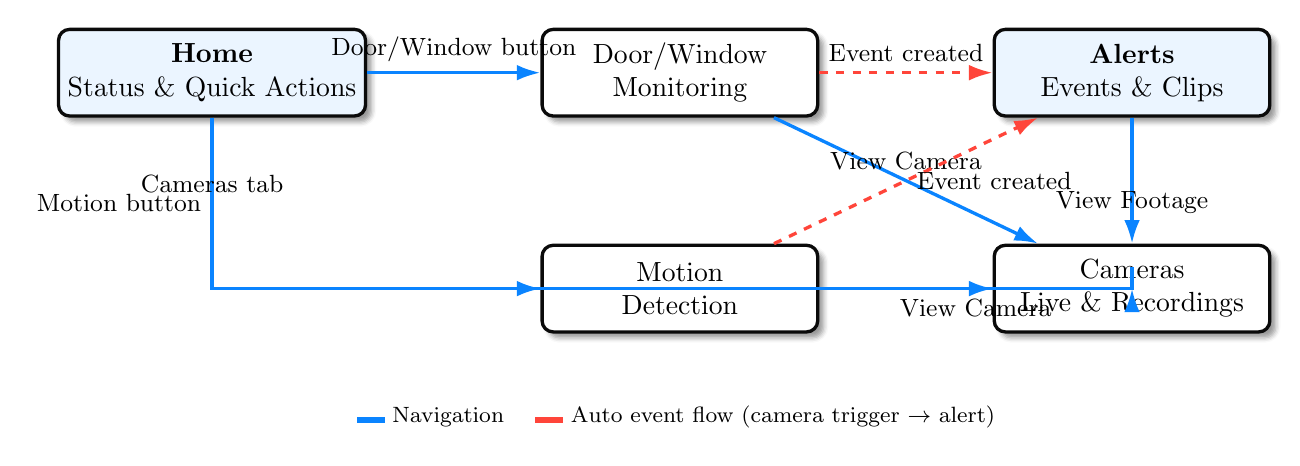
\begin{tikzpicture}[
    node distance=1.6cm and 2.2cm,
    box/.style={rounded corners, draw=ink, very thick, fill=white, blur shadow, minimum width=3.5cm, minimum height=1.1cm, align=center},
    arr/.style={-{Latex[length=3mm,width=2mm]}, very thick, draw=primary}
  ]

  \node[box, fill=primary!8] (home) {\textbf{Home}\\Status \& Quick Actions};
  \node[box, right=of home] (dw) {Door/Window\\Monitoring};
  \node[box, below=of dw] (motion) {Motion\\Detection};
  \node[box, right=of dw, fill=primary!8] (alerts) {\textbf{Alerts}\\Events \& Clips};
  \node[box, below=of alerts] (cameras) {Cameras\\Live \& Recordings};

  \draw[arr] (home) -- node[above]{\small Door/Window button} (dw);
  \draw[arr] (home) |- node[pos=0.25, left]{\small Motion button} (motion);
  \draw[arr] (home) |- node[pos=0.25, above]{\small Cameras tab} (cameras);
  \draw[arr] (dw) -- node[above]{\small View Camera} (cameras);
  \draw[arr] (motion) -| node[pos=0.25, below]{\small View Camera} (cameras);
  \draw[arr, dashed, draw=accent] (dw) -- node[above]{\small Event created} (alerts);
  \draw[arr, dashed, draw=accent] (motion) -- node[right]{\small Event created} (alerts);
  \draw[arr] (alerts) -- node[below]{\small View Footage} (cameras);

  % Legend
  \node[below=0.8cm of motion, align=left] (legend) {\footnotesize
    \textcolor{primary}{\rule{10pt}{2pt}}~Navigation \quad
    \textcolor{accent}{\rule{10pt}{2pt}}~Auto event flow (camera trigger $\rightarrow$ alert)
  };
  \end{tikzpicture}%
  }

  \caption{Navigation and event-driven flow including camera auto-trigger.}
\end{figure}

%\subsubsection{Technical Implementation}
\subsubsection{Platforms}
Cross-platform mobile app using \textbf{Flutter}.

\subsubsection{Communication}
\begin{itemize}
  \item \textbf{MQTT:} Low-latency sensor updates (\texttt{/home/zone1/door}, \texttt{/home/livingroom/motion}).
  \item \textbf{HTTPS REST API:} Event log queries, user actions, and recording retrieval.
  \item \textbf{WebRTC/RTSP:} Live video; recordings stored in cloud object storage.
\end{itemize}

\subsubsection{Backend}
Cloud microservices handle device registry, auth, and event processing. All traffic is encrypted (TLS 1.2+).

\subsubsection{Security}
\begin{itemize}
  \item \textbf{Authentication:} OAuth~2.0 with optional two-factor.
  \item \textbf{Authorization:} Role-based access (Owner, Family, Guest).
  \item \textbf{Privacy:} Encrypted video at rest; signed URLs for clip access; automatic redaction options.
\end{itemize}

\subsubsection{Figures}
App Mockup
\begin{figure}[h]
  \centering
  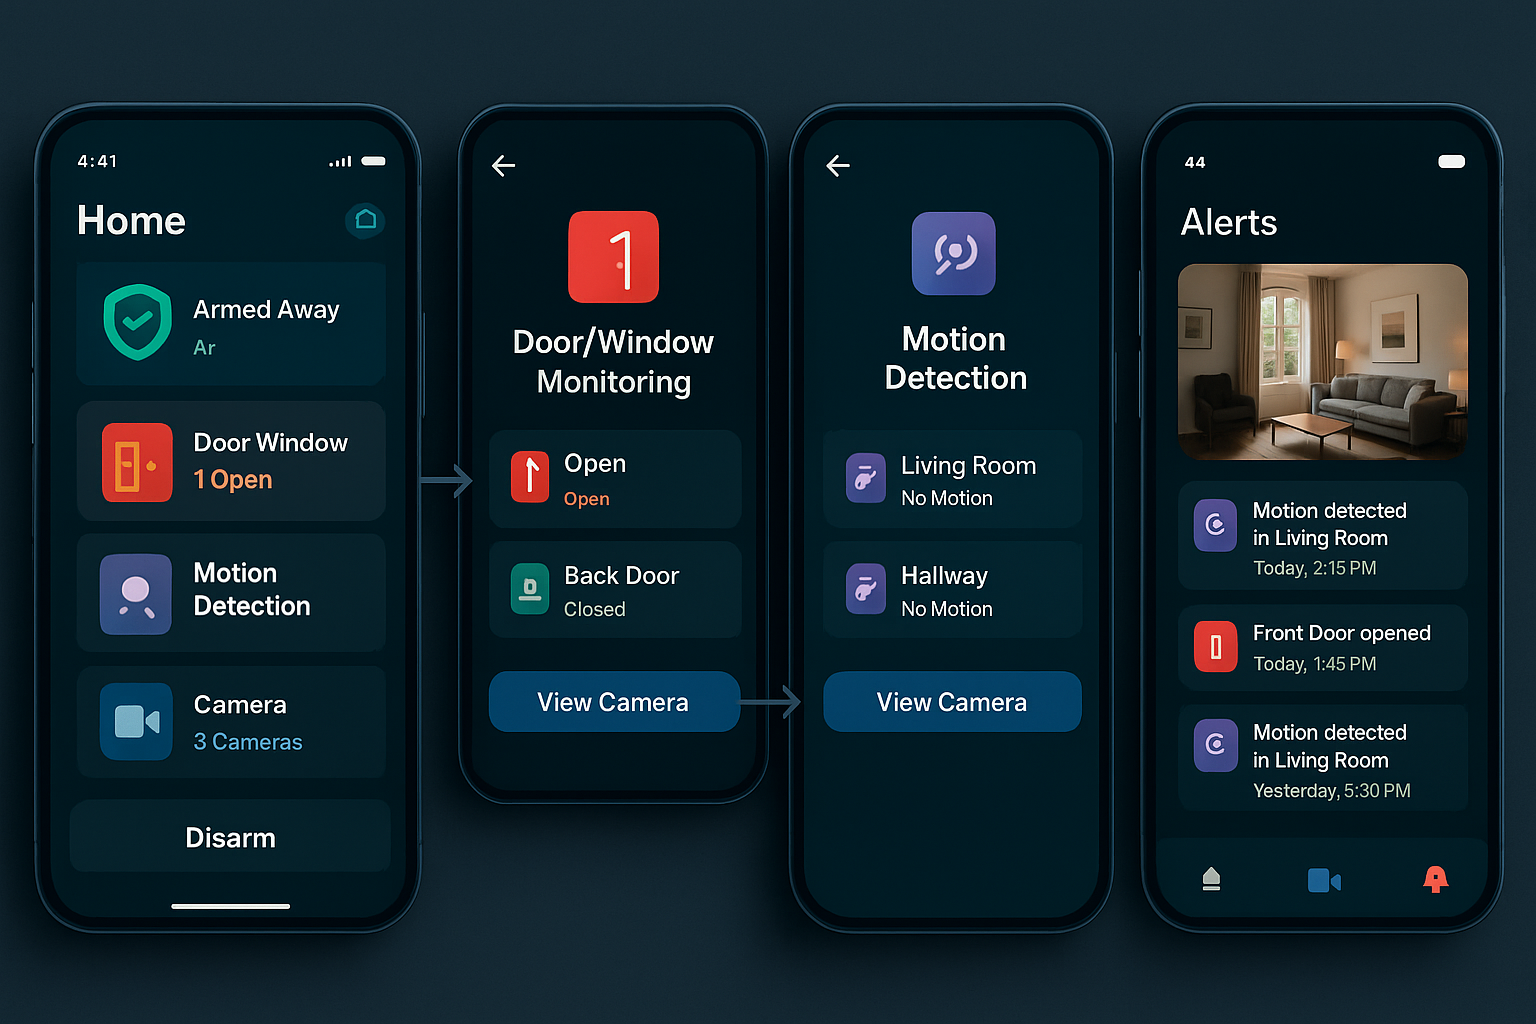
\includegraphics[width=\linewidth]{AppMockup.png}
  \caption{Smart Home Security app mockups showing Home, Door/Window, Motion, and Alerts with camera thumbnails.}
\end{figure}

\subsubsection{Traceability (Features to Screens)}
\begin{center}
\begin{tabularx}{\linewidth}{@{}lX@{}}
\toprule
\textbf{Requirement} & \textbf{UI Location} \\\midrule
Door/Window Monitoring & Home tile; Door/Window page (\emph{View Camera}) \\
Motion Detection & Home tile; Motion page (\emph{View Camera}) \\
Camera Integration & Cameras page; Alerts thumbnails; auto-trigger from events \\
Real-time Alerts & Alerts feed; push notifications \\
Remote Control & Home quick actions; Devices page (Siren/Lights) \\
Monitoring Dashboard & Home overview; Events log on Alerts \\
\bottomrule
\end{tabularx}
\end{center}

% --- Person 5 (HAMSA) writes here ---
% A. Describe the user-facing application (e.g., a mobile app).
% B. Include user interface mockups and describe functionality (dashboard, notifications, etc.).


\section{Conclusion}
% Summarize the key design decisions made throughout the 10 steps.
% Reiterate the capabilities of the proposed system.
% Briefly mention future work or potential improvements.


\section*{Acknowledgment}
The authors wish to thank the teaching staff of the Computer and Systems Engineering Department at Ain Shams University for their guidance and support throughout this project.


%%%%%%%%%%%%%%%%%%%%%%%%%%%%%%%%%%%%%%%%%%%%%%%%%%%%%%%%%%%%%%%%%%%%%%%%%%%%%%%%
% --- BIBLIOGRAPHY SECTION ---
% This tells LaTeX to use the 'IEEEtran' style for references
% and to look for them in the 'references.bib' file.
%%%%%%%%%%%%%%%%%%%%%%%%%%%%%%%%%%%%%%%%%%%%%%%%%%%%%%%%%%%%%%%%%%%%%%%%%%%%%%%%
\bibliographystyle{IEEEtran}
\bibliography{references}

\end{document}